\newpage
\appendix
\newpage

\pagenumbering{gobble}

\captionsetup[figure]{font=small,skip=0pt}
\etocdepthtag.toc{mtappendix}
\etocsettagdepth{mtchapter}{none}
\etocsettagdepth{mtappendix}{subsection}
\etoctocstyle{1}{Appendix - Contents}
\tableofcontents
\pagestyle{plain}

\newpage
\pagenumbering{arabic}
\chapter{Detailed Explanations and Supplementary Results}
In this chapter, the detailed explanations of the concepts discussed in the main text and present supplementary results that contribute to a clearer overview of the key outcomes of this thesis. These additional findings provide valuable context and insights that complement the primary research findings.

\section{Quaternions to Euler Angles}
\label{sec:Q2E}
Even though Euler angles are used to represent rotations, the transmission of two poses are calculated by Quaternion, which is a mathematical construct that extends the notion of complex numbers to four dimensions. They comprise four components: a scalar part represented by $w$, and a vector component denoted as $\vec{v}=(x, y, z)$. Quaternions are expressed as:
$$q = w + xi + yj + zk$$
where $x$, $y$, $z$, and $w$ are real numbers, and $i$, $j$, and $k$ are three imaginary units that satisfy the following multiplication rules: $i^2 = j^2 = k^2 = ijk = -1$. This approach involves establishing the initial pose of the robot as a quaternion and subsequently updating the current pose through sensors like accelerometers and gyroscopes. By computing the difference between the initial and current poses, the rotational component of the transformation can be extracted. This rotational component is often represented as a 3x3 rotation matrix $R$, which can then be used to derive the Euler angles 'yaw', 'pitch', and 'roll', providing insights into the robot's orientation in three-dimensional space. 
$$ R = \begin{bmatrix}
1 - 2(y^2 + z^2) & 2(xy - wz) & 2(xz + wy) \\
2(xy + wz) & 1 - 2(x^2 + z^2) & 2(yz - wx) \\
2(xz - wy) & 2(yz + wx) & 1 - 2(x^2 + y^2)
\end{bmatrix}
$$
The conversion from the rotation matrix 'R' to Euler angles 'yaw', 'pitch', and 'roll' involves the following mathematical expressions:
\begin{align*}
\text{yaw (Y)} & = \text{atan2}(R_{21}, R_{11}) \\
\text{pitch (X)} & = -\text{asin}(R_{31}) \\
\text{roll (Z)} & = \text{atan2}(R_{32}, R_{33})
\end{align*}

\section{Kalman Filter Update}
\label{sec:kf}
The Kalman filter, a fundamental tool in state estimation for dynamic systems, continuously refines its state estimate in the presence of noisy measurements. This section provides an overview of the Kalman filter's update process, shedding light on its predictive and corrective steps.

\textbf{State Transition Model (Predictive Step):}
In the predictive step, the Kalman filter employs the system's dynamics to forecast the next state ($x_{k|k-1}$) based on the previous state estimate ($x_{k-1|k-1}$). This forecast hinges on a linear transformation captured by the state transition matrix ($A$):
\begin{equation*}
x_{k|k-1} = A \cdot x_{k-1|k-1} + B u_{k|k}
\end{equation*}

The state covariance ($P_{k|k-1}$) is also updated to account for the inherent uncertainty in this prediction:
\begin{equation*}
P_{k|k-1} = A \cdot P_{k-1|k-1} \cdot A^T + Q
\end{equation*}
Here, $Q$ represents the process noise covariance matrix, characterizing the uncertainty introduced by the system dynamics.

\textbf{Measurement Update (Corrective Step):}
In the corrective step, measurements ($z_k$) are incorporated into the state estimate to enhance its accuracy. The Kalman gain ($K_k$) is computed to determine the weight assigned to the measurement versus the prediction:
\begin{equation*}
K_k = P_{k|k-1} \cdot H^T \cdot (H \cdot P_{k|k-1} \cdot H^T + R)^{-1}
\end{equation*}
In this equation, $H$ represents the measurement matrix, mapping the state to the measurement space. The measurement noise covariance matrix ($R$) captures the uncertainty associated with sensor measurements.

Leveraging the Kalman gain, the state estimate and its covariance are updated as follows:
\begin{align*}
x_{k|k} = x_{k|k-1} + K_k \cdot (z_k - H \cdot x_{k|k-1}) \
P_{k|k} = (I - K_k \cdot H) \cdot P_{k|k-1}
\end{align*}
In these equations, $I$ denotes the identity matrix. The Kalman filter's iterative process continually refines the state estimate and its associated uncertainty, making it a powerful tool for state estimation in the presence of noise and uncertainty.

\section{ANCOVA}
\label{Sec:ANCOVA}
ANCOVA is a powerful statistical tool that allows us to rigorously assess the impact of our independent variables while controlling for covariates.  In our case, the covariate of interest is the reference walking speed ($v_{ref}$), which could potentially influence the dependent variables. The \ac{DoF}  represent the number of values in the final calculation of a statistic that are free to vary, and Sum of Squares(Sum Sq) quantifies the variability in our data and helps us understand the contribution of different factors to that variability. Mean square is the average of the sum of squares values. It's a key statistic in ANCOVA, as it allows us to compare the variation explained by the model to the unexplained variation (error). We calculate Mean Square Model (MSM) and Mean Square Error (MSE). The F-statistic is a crucial test statistic in ANCOVA. It quantifies the ratio of the variation explained by the model (MSM) to the unexplained variation (MSE). The F-statistic is used to determine whether the independent variable (in our case, the RL method: MBRL or MFRL) has a significant effect on the dependent variables. Probability (p) values associated with the F-statistic indicate the likelihood of observing such a statistic if the null hypothesis is true. In our case, a low p-value suggests that the RL method has a significant effect. The Pro>F value indicates the probability of obtaining an F-statistic as extreme as the one observed, given that the null hypothesis is true. Here is how does these measures calculated:

\begin{itemize}
    \item \ac{DoF}: (For the model) $\text{DoF}_{\text{Model}} = \text{Number of groups (RL methods)} - 1$, (For the error) $\text{DoF}_{\text{Error}} = \text{Total number of observations} - \text{DoF}_{\text{Model}} - 1$
    \item Sum of Squares (Sum Sq):$\text{SST} = \sum(y_i - \bar{y})^2$, where $y_i$ is each individual data point, and $\bar{y}$ is the overall mean.
    \item Model Sum of Squares (SSM): $\text{SSM} = \sum(n_i)(\bar{y}_i - \bar{y})^2$,  where $n_i$ is the number of observations in each group.
    \item Error Sum of Squares (SSE): $\text{SSE} = \sum\sum(y_{ij} - \bar{y}_i)^2$, where $y_{ij}$ is each individual data point within each group.
    \item Mean Square Model (MSM): $\text{MSM} = \frac{\text{SSM}}{\text{DoF}_{\text{Model}}}$
    \item Mean Square Error (MSE): $\text{MSE} = \frac{\text{SSE}}{\text{DoF}_{\text{Error}}}$
    \item F-statistic: $\text{F-statistic} = \frac{\text{MSM}}{\text{MSE}}$
\end{itemize}

\section{Single Step Prediction of two NNs}
\begin{figure}[htb]
    \centering
    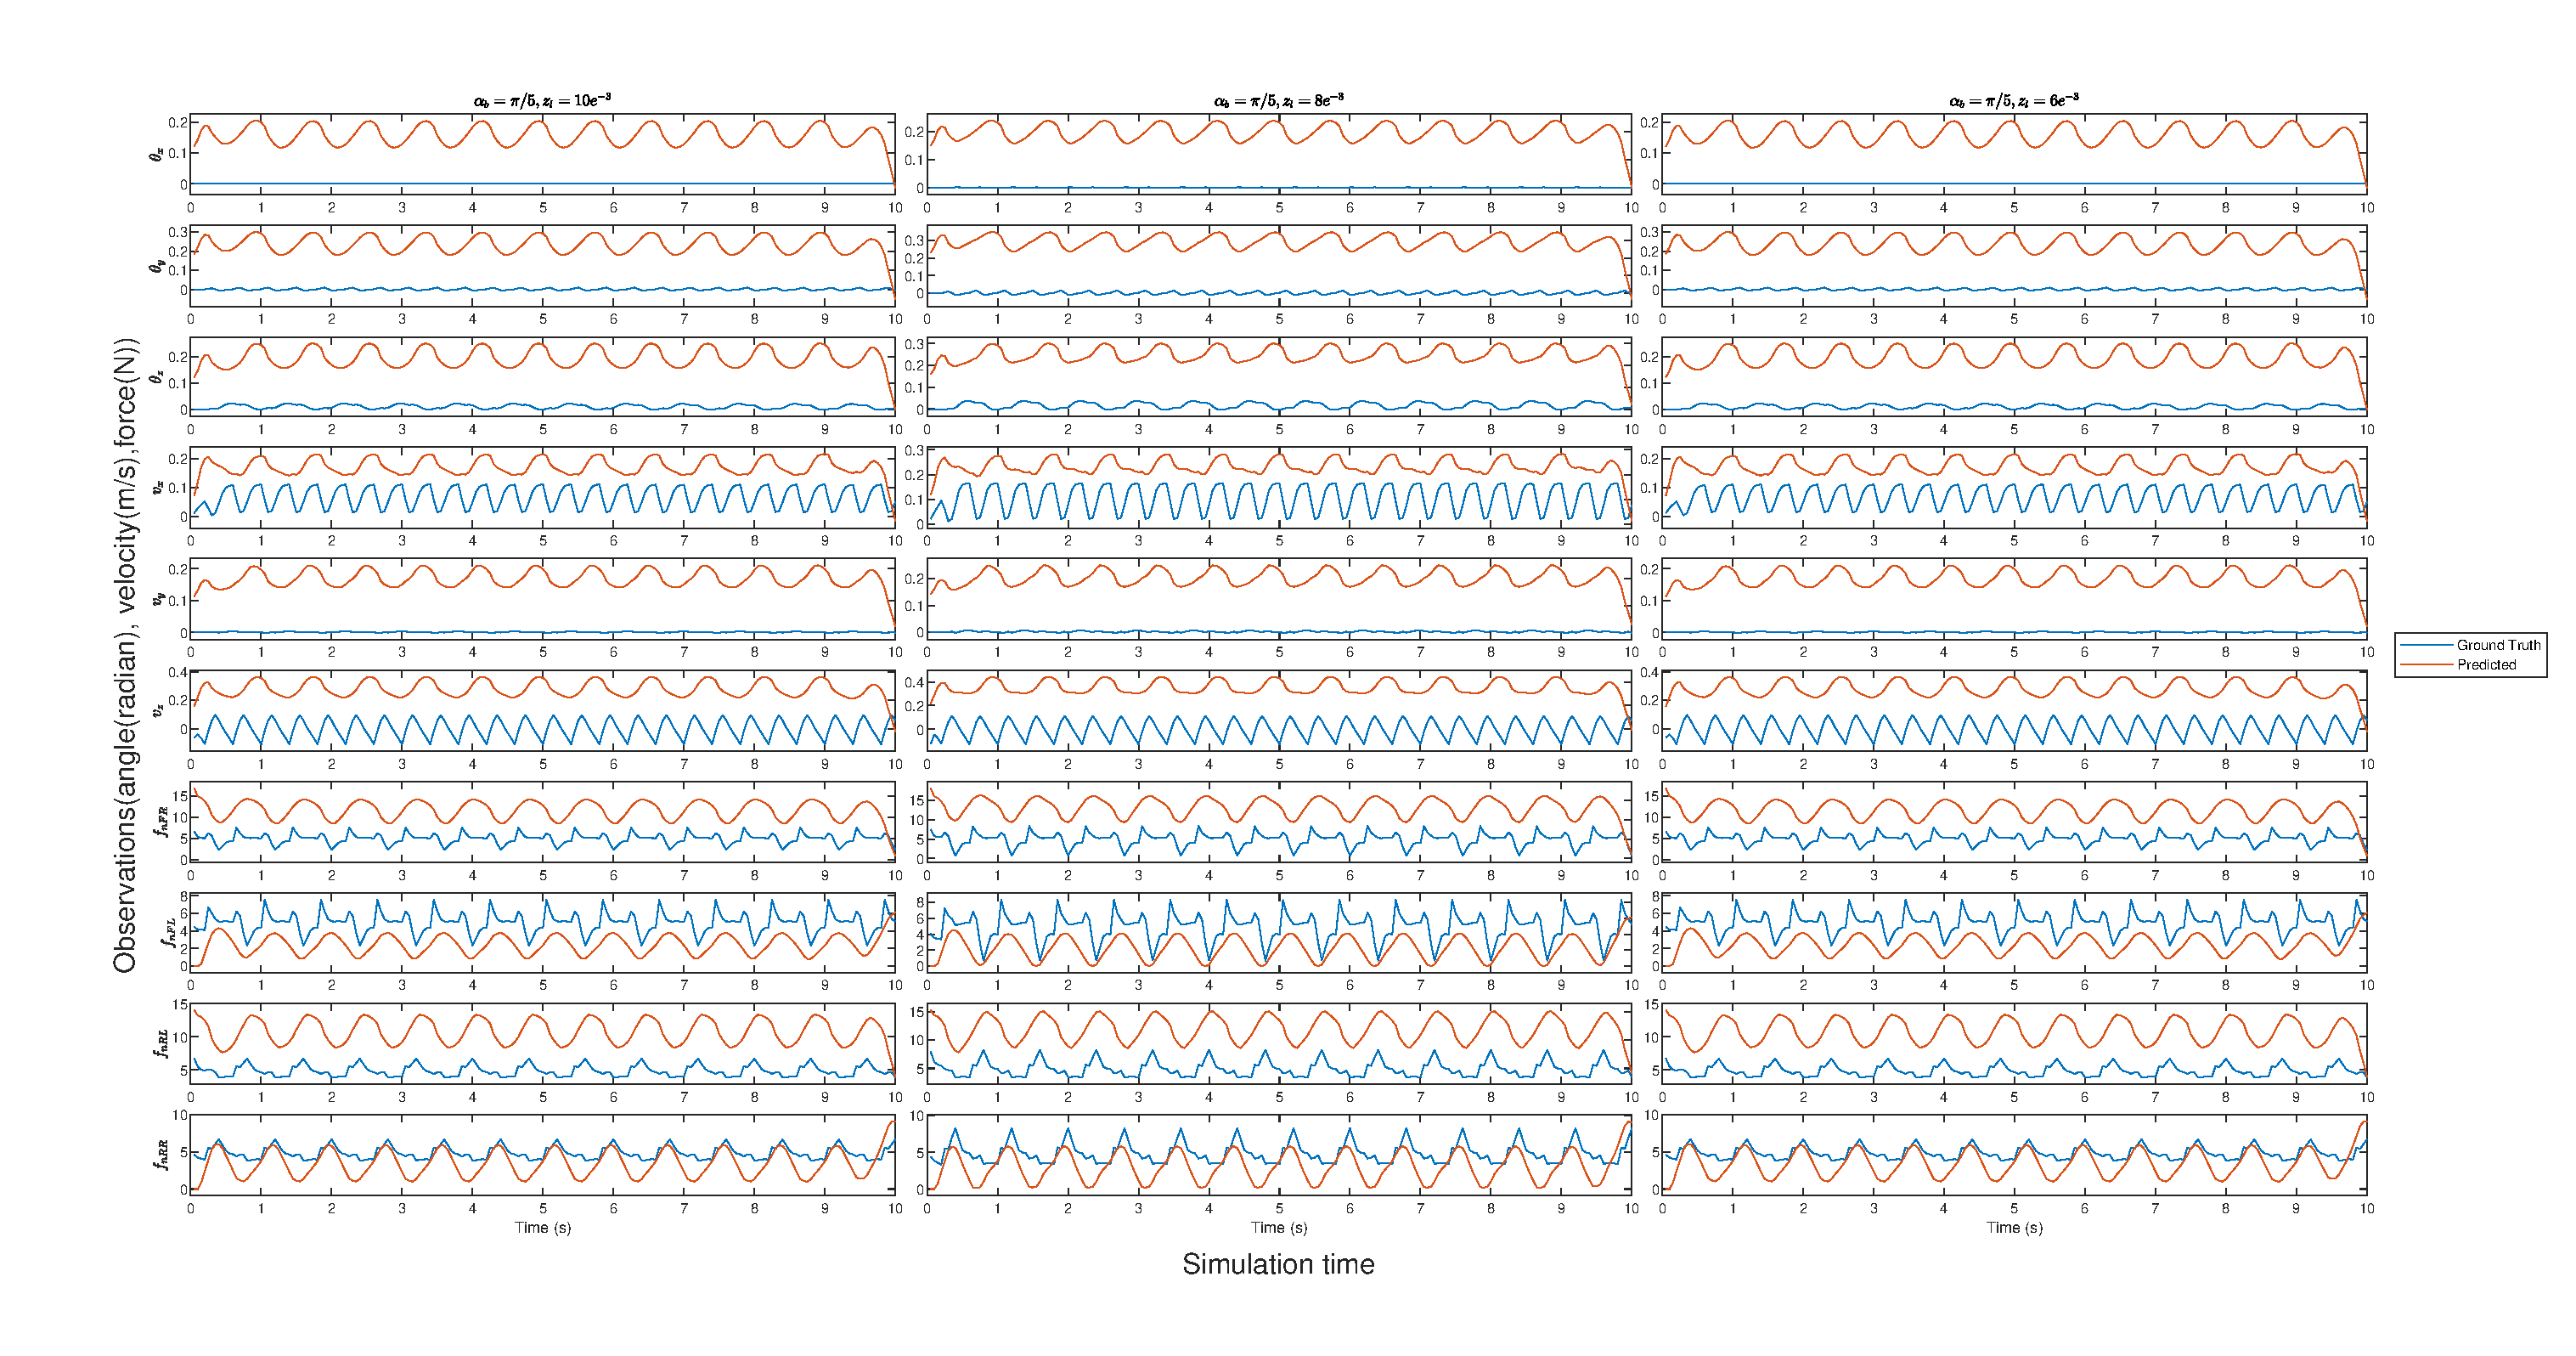
\includegraphics[width=\linewidth]{img/AppA/lstm_pred.eps}
    \caption{Single step prediction test of LSTM network}
    \label{fig:lstm_test}
\end{figure}

\begin{figure}[htb]
    \centering
    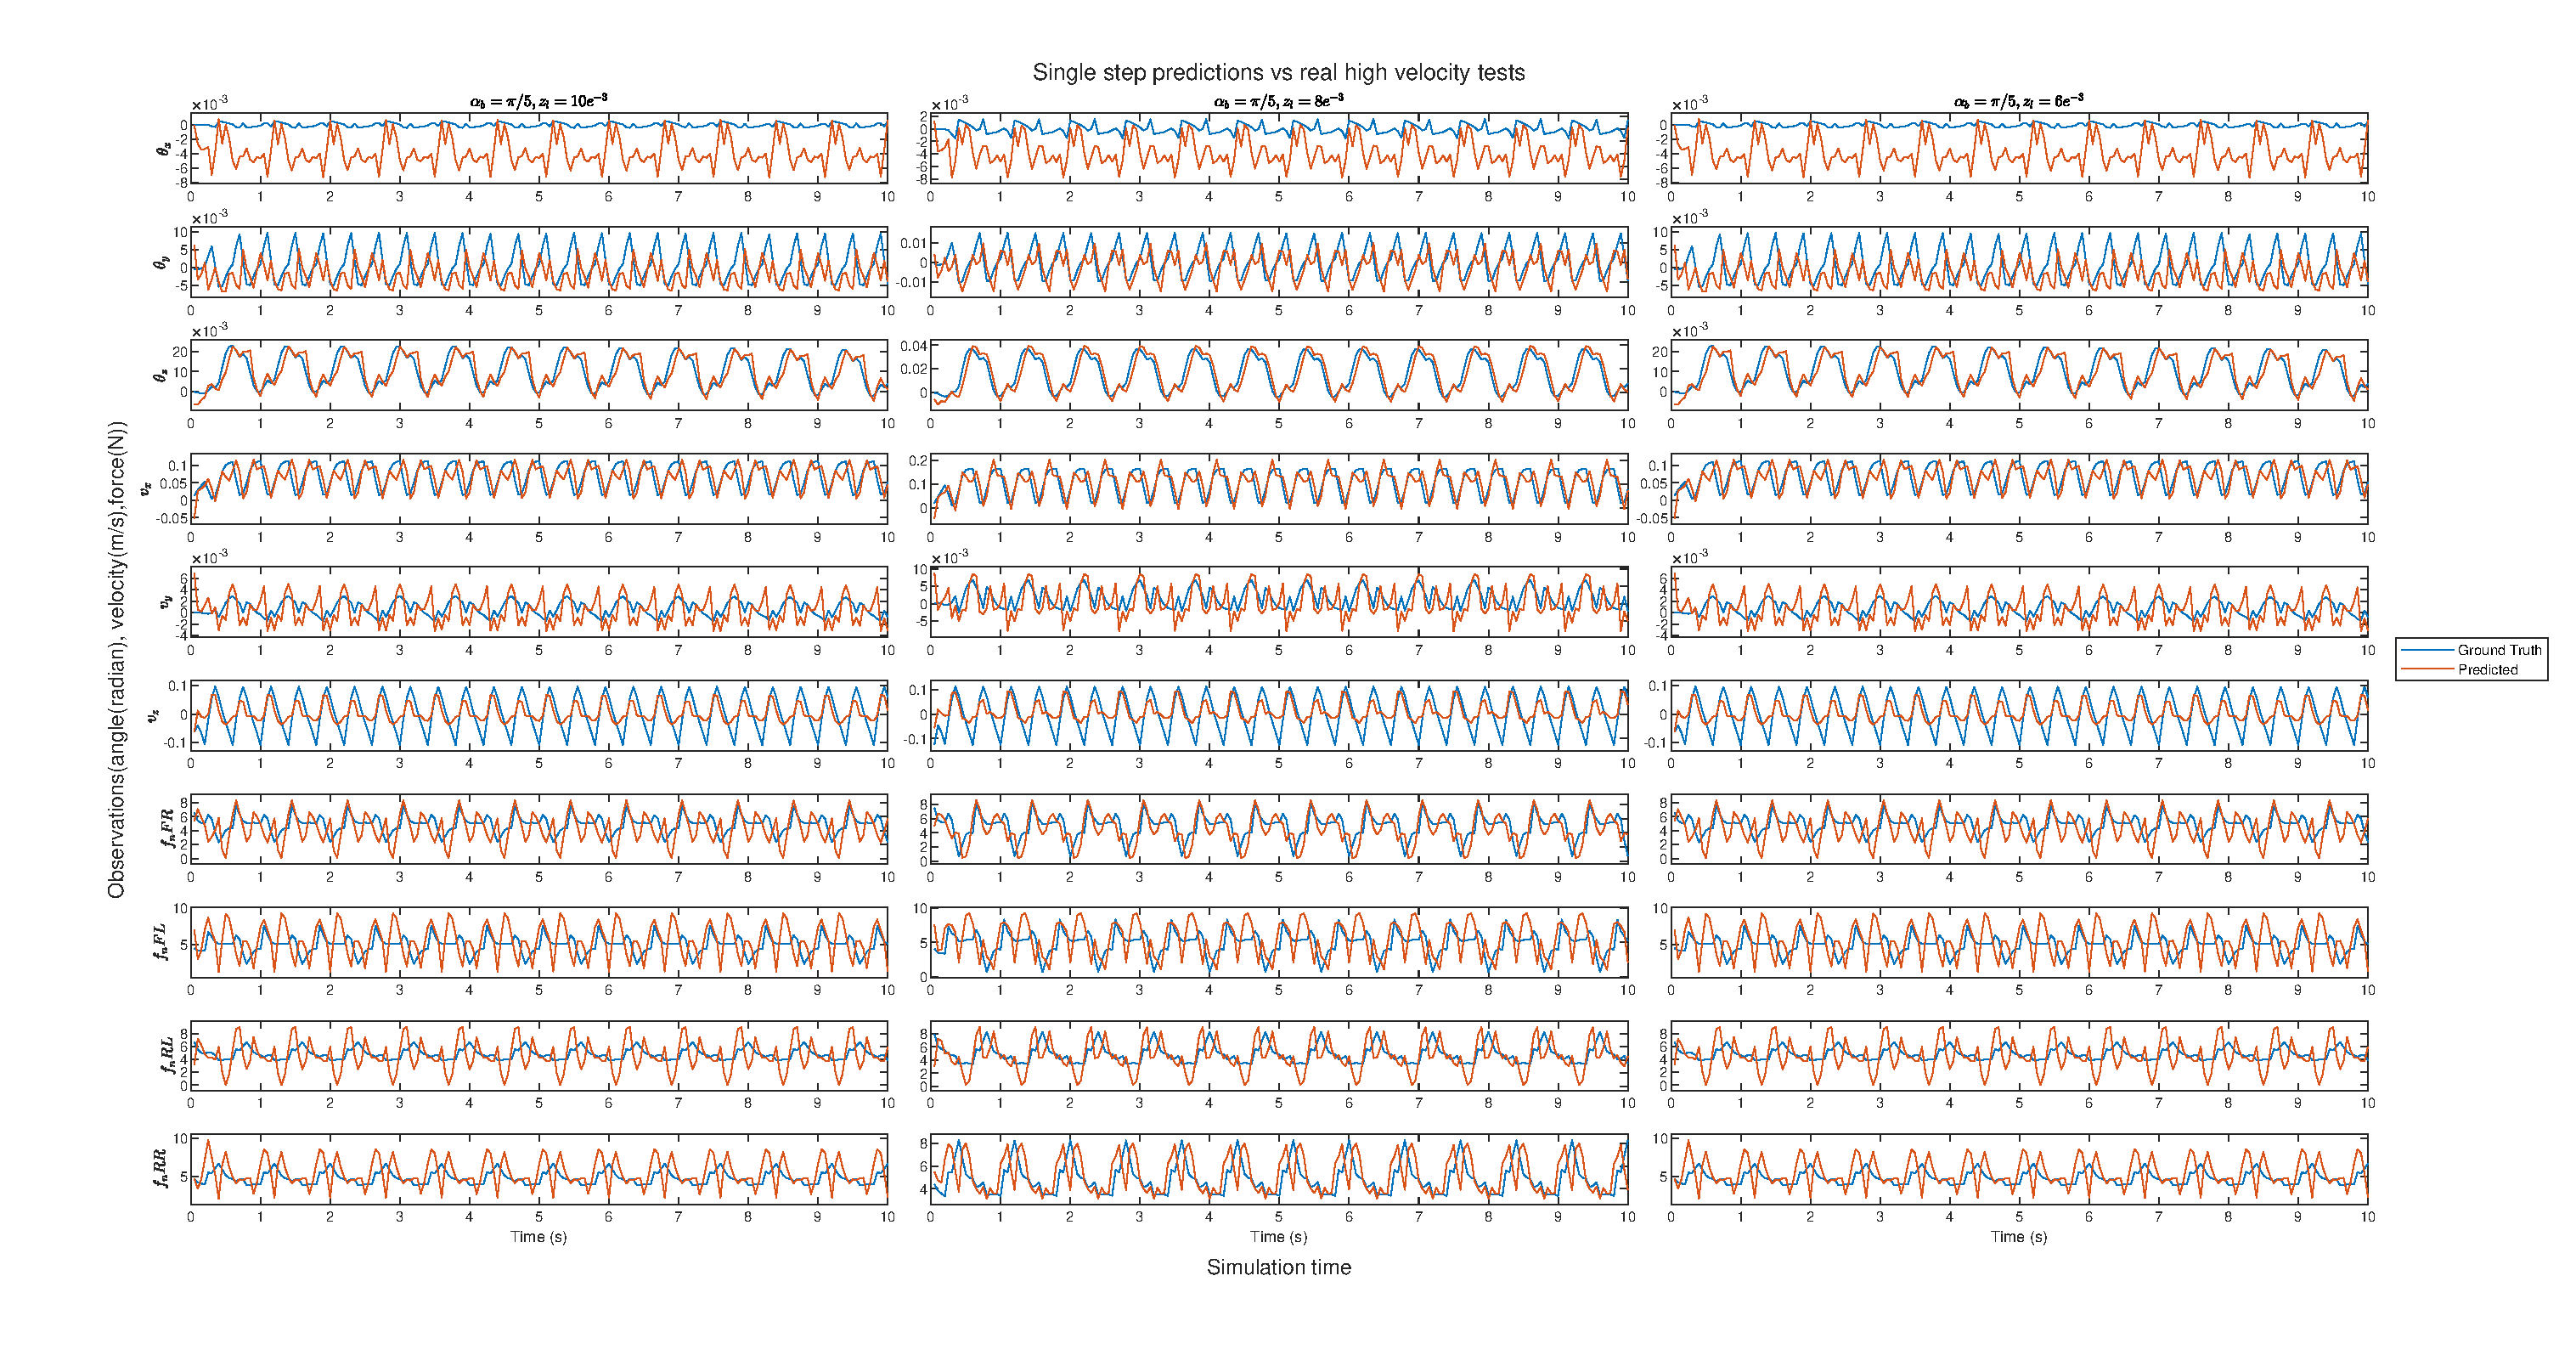
\includegraphics[width=\linewidth]{img/AppA/model_all.eps}
    \caption{Single step prediction test of DNN}
    \label{fig:DNN_test}
\end{figure}

\section{Expert Gait Walking in Validation}
\begin{figure}[htb]
    \centering
    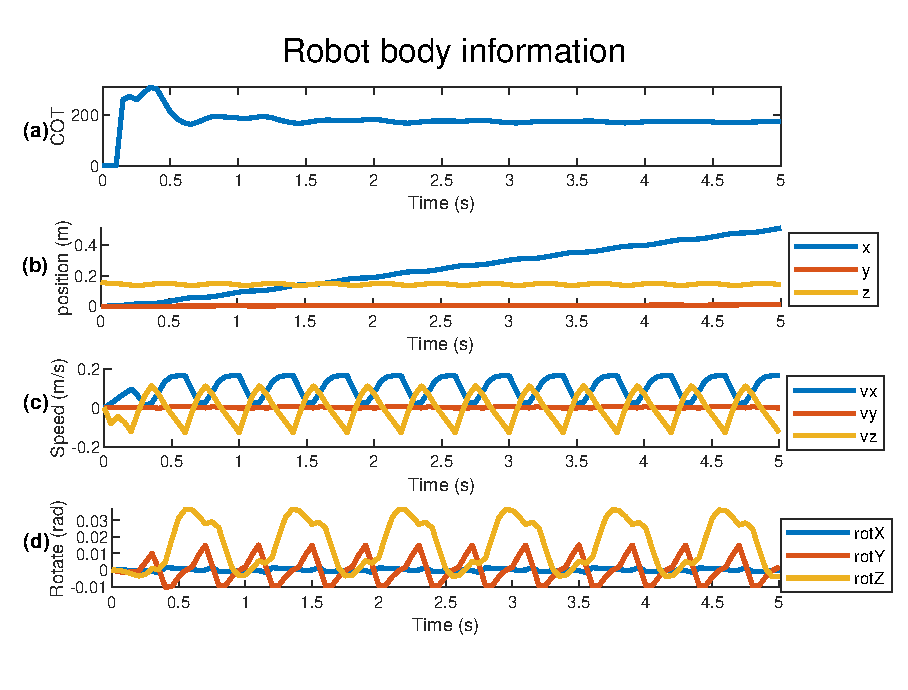
\includegraphics[width=\linewidth]{img/AppA/expert_val.eps}
    \caption{Expert Gait Tested in Validation Results. (a) COT of the robot while walking; (b) Distance traveled along the $x$, $y$, and $z$ axis; (c) Speed of the robot along the $x$, $y$, and $z$ axis; (d) Orientation of the robot along the $x$, $y$, and $z$ axis.}
    \label{fig:expert_val}
\end{figure}


\chapter{Additional Showcases}
In this chapter, the main the source code and block diagrams implemented in Simulink is provided, together with some videos of validating the trained agents. These elements play a crucial role in this thesis, enabling the replication of experiments, validation of results, and the potential for further advancements in our work.

\section{Main Code of SoftQ}
There are two main codes used for controlling and running the robot, Python code are designed for the main brain. Simulink generated C code for controller, but other than that, main code need for training MBRL and MFRL are shown.
\subsection*{Python Code for SoftQ}
The Python code for SoftQ can be found in here: \href{https://github.com/n7729697/KTH-MasterThesis/blob/main/code/SoftQ_optimized.py}{\faGithub\, \underline{Python Code}}

\subsection*{Matlab Code for MBRL}
\label{code:mbrl}
The Matlab code for MBRL training can be found in here: \href{https://github.com/n7729697/KTH-MasterThesis/blob/main/code/MBRLmain.mlx}{\faGithub\,\underline{MBRLmain Code}}
The Matlab code for creating RL training agent can be found in here: \href{https://github.com/n7729697/KTH-MasterThesis/blob/main/code/createAgent.mlx}{\faGithub\,\underline{createAgent Code}}

\section{Block Diagrams from Simulink}
\subsection*{Block Diagrams for Collecting Stochastic Data.}
The block diagrams for MBRL training and simulation in simulink could be found in here: \href{https://github.com/n7729697/KTH-MasterThesis/blob/main/img/AppB/ModelRobot.pdf}{\faGithub\,\underline{ Stochastic data acquisition block diagram}}
\subsection*{Block Diagrams for MBRL}
The block diagrams for MBRL training and simulation in simulink could be found in here: \href{https://github.com/n7729697/KTH-MasterThesis/blob/main/img/AppB/it.pdf}{\faGithub\,\underline{ MBRL training block diagram}}
\subsection*{Block Diagrams for Continue Training and MFRL}

\subsection*{Block Diagrams for Simulink Controller}

\section{Video from Simulation and Field Tests}
\label{video}